%%----------------------------------------------------------------------------
%% Presentatie HoGent Bedrijf en Organisatie
%%----------------------------------------------------------------------------
%% Auteur: Bert Van Vreckem [bert.vanvreckem@hogent.be]

\documentclass[notes]{beamer} 

%==============================================================================
% Aanloop
%==============================================================================

%---------- Packages ----------------------------------------------------------

\usepackage{graphicx,multicol}
\usepackage{comment,enumerate,hyperref}
\usepackage{amsmath,amsfonts,amssymb}
\usepackage{tikz}
\usepackage[english]{babel}
\usepackage[utf8]{inputenc}
\usepackage{multirow}
\usepackage{eurosym}
\usepackage{listings}
\usepackage[T1]{fontenc}
\usepackage{lmodern}
\usepackage{textcomp}
\usepackage{framed}
\usepackage{wrapfig}
\usepackage{pgfpages}



%---------- Configuratie ------------------------------------------------------

\usetikzlibrary{arrows,shapes,backgrounds,positioning,shadows}

\usetheme{hogent}

%---------- Commando-definities -----------------------------------------------

\newcommand{\tabitem}{~~\llap{\textbullet}~~}

%---------- Info over de presentatie ------------------------------------------

\title[Intro]{Creative Thinking}
\author{Jens Buysse}
\date{\today}

%==============================================================================
% Inhoud presentatie
%==============================================================================

\begin{document}

%---------- Front matter ------------------------------------------------------

% Dia met het HoGent logo
\HoGentLogo

% Titeldia met faculteitslogo
\titleframe

%---------- Inhoud ------------------------------------------------------------

\begin{frame}
  \frametitle{Inhoud}

  \tableofcontents
\end{frame}

\section{What is creative thinking}

\sectionframe{\begin{center}
		
\includegraphics[height=0.6\textheight]{img/intro.jpg}
\end{center}}

\begin{frame}{What is thinking?}
	\begin{center}
		\begin{figure}
			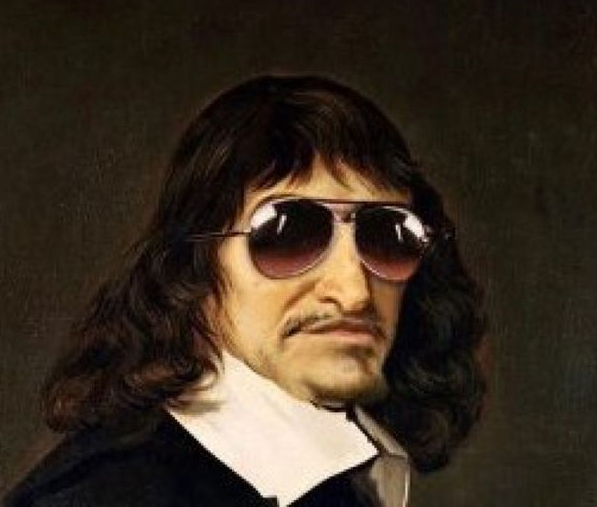
\includegraphics[height=0.6 \textheight]{img/rene.jpg}
		\end{figure}
	\end{center}
\note{Descartes tries to give a definition of "thought" in principle I.9. By "thought" he tells us, he means to refer to anything marked by awareness or consciousness. This does not just include reasoning or other such intellectual activities but also imagining, sensing, willing, believing, doubting, hoping, dreading, and all other mental operations.}
\end{frame}


\begin{frame}{What is thinking?}
	\begin{figure}
		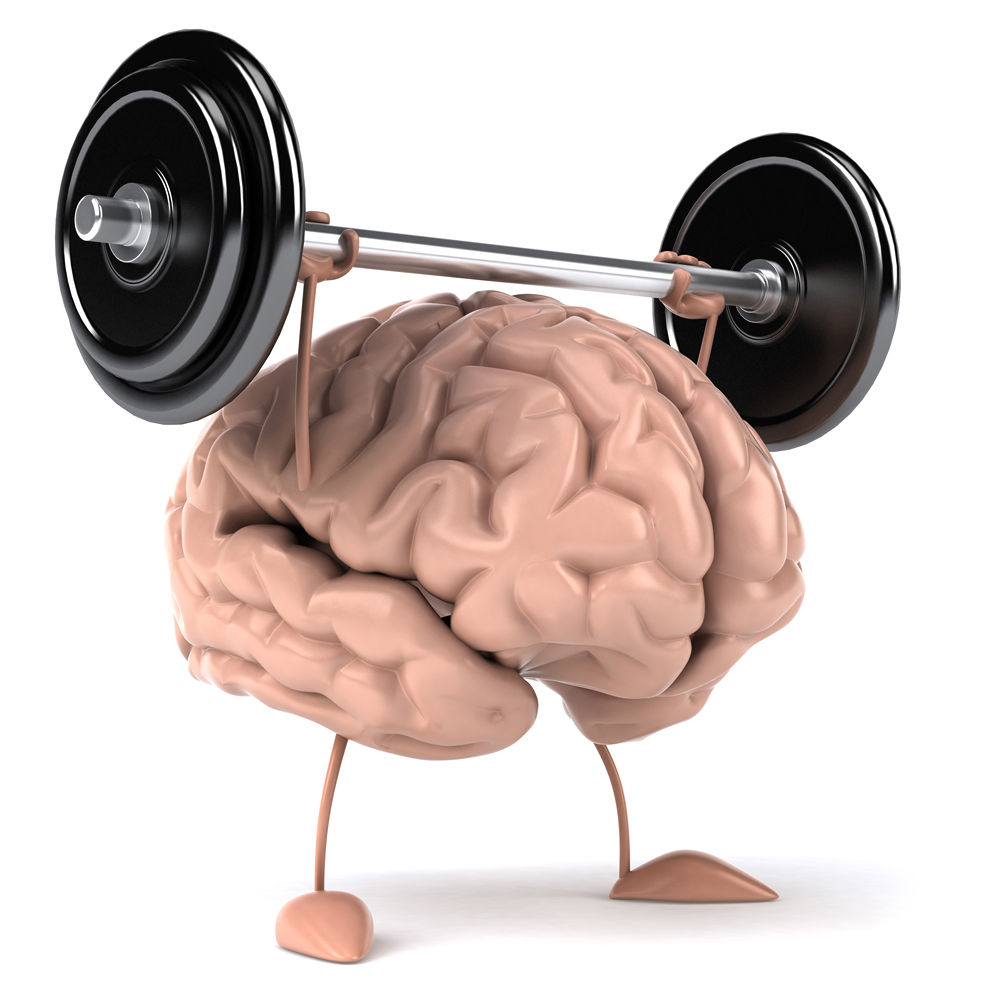
\includegraphics[height=0.6\textheight]{img/brain.jpg}
	\end{figure}
\note{Your brain is made of approximately 100 billion nerve cells, called neurons. Neurons have the amazing ability to gather and transmit electrochemical signals (up to several feet or a few meters) and send messages to each other. Dendrites or nerve endings. These small, branchlike projections of the cell make connections to other cells and allow the neuron to talk with other cells or perceive the environment. Dendrites can be located on one or both ends of a cell.}
\end{frame}

\begin{frame}{What is thinking?}
	\href{http://www.youtube.com/watch?v=BGPGknpq3e0}{Is \underline{this} an example of thinking?}
\end{frame}

\begin{frame}{Excercise}
	\brightbox{Take a sheet of paper and draw an \textcolor{HoGentAccent6}{alien}}
	\note{Most of the studenst will have drawn a default alien with arms and legs and eyes. But why not a blob, or a dot, or just a line}
\end{frame}


\begin{frame}{What is \textcolor{HoGentAccent6}{creative} thinking?}
	\begin{figure}
		\includegraphics[width=10cm]{img/babydriving}
	\end{figure}
\end{frame}

\begin{frame}{What is \textcolor{HoGentAccent6}{creative} thinking?}
	\begin{figure}
		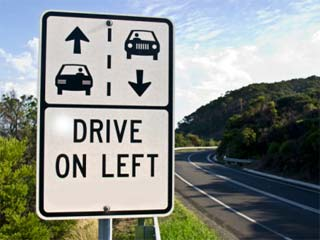
\includegraphics[width=8cm]{img/drive.jpg}
	\end{figure}
\end{frame}

\begin{frame}{What is \textcolor{HoGentAccent6}{creative} thinking?}
	\begin{itemize}
		\item Experience is the sum of patterns.
		\item Patterns which we have created througout or life
		\item \textcolor{HoGentAccent1}{Creative thinking} is trying to break these patterns which we are so accustomed to. 
	\end{itemize}

\begin{center}
	\begin{figure}
		
\includegraphics[width=5cm]{img/puzzel.jpg}
	\end{figure}
\end{center}
\end{frame}

\begin{frame}{Excercise}
	\begin{itemize}
		\item There is blood on the ceiling. There has been no muder of killing or accident. Nobody has played a trick on me. Can you suggest an explanaton. 
	\end{itemize}

\note{A mosquito bit me, landed on the ceiling and and I swatted it.}
\end{frame}

\begin{frame}{Excercise}
	\begin{itemize}
		\item There is a flash of light and a man dies. The man is not killed by any other person and he does not die of an illness like a heart attack \dots It is not suicide. Can you suggest an explanation?
	\end{itemize}
	
	\note{The man is a lion tamer, posing for a photo with the lion. Somebody took a picture and the lion reacted badly, so he gets mauled}
\end{frame} 

\begin{frame}{Excercise}
	\begin{itemize}
		\item An ordinary American Citizen with no passport on him visits over thirthy oreign countries in one day. He is welcomed in each country and leaves each one of his own accord?
	\end{itemize}
	
	\note{He is a mail courier who delivers packages to different foreign embassies in the embassies. The land of an embassy belongs to the country of the embassy, not the united states.}
\end{frame}

\section{Attitudes towards Creative Thinking}

\sectionframe{\begin{center}
		
\includegraphics[width=0.8\textwidth]{img/attitude.jpg}
\end{center}}	

\section{Creative techniques}

%---------- Back matter -------------------------------------------------------

\end{document}
